\documentclass[tikz,border=2mm]{standalone}
\usetikzlibrary{positioning,arrows.meta}
\usepackage{tikz}

\begin{document}
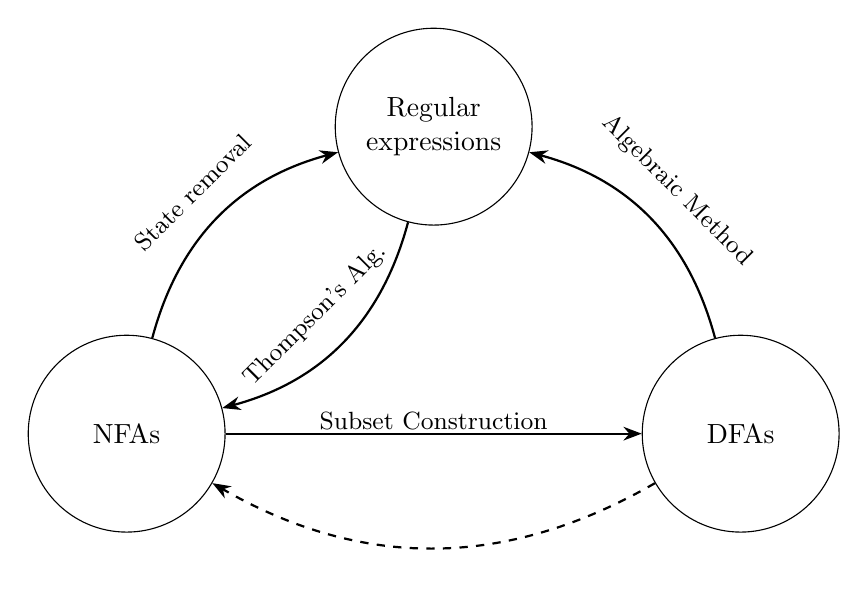
\begin{tikzpicture}[
	node distance=3cm,
    >=Stealth,
    main/.style={draw, circle, minimum size=2.5cm, align=center},
    cycle arrow/.style={->, thick},
    back arrow/.style={dashed,->, thick},
    edgelabel/.style={
      font=\small,
      midway,
      sloped,
      align=center,
      draw=none,
      fill=none,
      inner sep=1pt
    }
  ]

  % spread them out at explicit coords
  \node[main] (RE)  {Regular\\expressions};
  \node[main] (NFA) [below left=of RE]  {NFAs};
  \node[main] (DFA) [below right=of RE] {DFAs};

  % RE <-> NFA
  \draw[cycle arrow, bend left=30]
    (RE)  to node[edgelabel, above=3mm] {Thompson’s Alg.} (NFA);
  \draw[cycle arrow, bend left=30]
    (NFA) to node[edgelabel, above=3mm] {State removal} (RE);

  % RE <-> DFA
  \draw[cycle arrow, bend right=30]
    (DFA) to node[edgelabel, above=3mm] {Algebraic Method} (RE);

  % NFA -> DFA (subset)
  \draw[cycle arrow]
    (NFA) to node[edgelabel, above] {Subset Construction} (DFA);

  % DFA -> NFA (dashed back‐inclusion)
  \draw[back arrow, bend left=30]
    (DFA) to node[edgelabel, below] {} (NFA);

\end{tikzpicture}
\end{document}


